\documentclass[../thesis.tex]{subfiles}

\begin{document}

\renewcommand*\thesection{\arabic{section}}

\section{Đặt vấn đề}

Trong những năm gần đây, với sự tăng trưởng mạnh mẽ về lượng dữ liệu và khả năng xử lý tính toán của CPU/GPU, máy học (Machine Learning) mà cụ thể là học tập sâu (Deep Learning) đã đi dần đi vào cuộc sống con người qua những ứng dụng của thị giác máy tính (Computer Vision), xử lý ngôn ngữ tự nhiên (Natural Language Processing) hay hệ thống gợi ý (Recommendation System). Một trong những ứng dụng quan trọng của học tập sâu được nhắc đến nhiều nhất là xe tự hành.

Hệ thống tự lái của xe tự hành là sự kết hợp của nhiều mô hình máy học, học tập sâu, trong đó có mô hình nhận dạng đối tượng (Object Detection) giúp phát hiện các đối tượng xuất hiện trên đường bao gồm các phương tiện giao thông, biển báo giao thông và người đi bộ. Một bài toán được đặt ra ở đây là làm thế nào để có thể tạo ra một mô hình đủ tốt để phát hiện (detect) và phân loại (classify) các đối tượng trên đường mà vẫn hoạt động với tốc độ có thể chấp nhận được trên một phần cứng giới hạn.  

Bài toán nhận dạng đối tượng (Object Detection) là sự kết hợp giữa bài toán phân lớp (classification) và bài toán hồi quy (regression). Với bài toán phân lớp, ta luôn giả thử rằng dữ liệu đầu vào luôn chứa đối tượng ở trong đó và chỉ có duy nhất một đối tượng nằm hoàn toàn trong ảnh đầu vào, nhiệm vụ của thuật toán phân lớp là cho biết đối tượng trong ảnh đó thuộc lớp nào. Tuy nhiên, với bài toán nhận dạng đối tượng, ta cần phải giải quyết hai vấn đề, đầu tiên là xác định xem đối tượng xuất hiện ở vị trí nào trên ảnh, mỗi ảnh có thể chứa nhiều đối tượng và xác định xem các đối tượng ấy thuộc những lớp nào.

\begin{figure}[H]
    \centering
    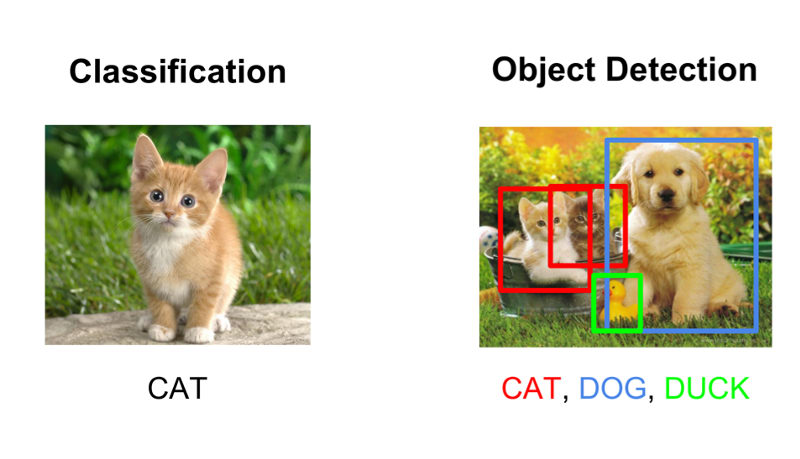
\includegraphics[width=\linewidth]{classification_vs_object_detection.jpg}
    \caption{Bài toán phân lớp và bài toán nhận dạng đối tượng}\label{classification_vs_object_detection}
\end{figure}

\section{Lịch sử giải quyết vấn đề}

Đã có rất nhiều các giải pháp được đưa ra nhằm giải quyết bài toán được nêu ở trên, có thể kể đến là sử dụng đặc trưng HOG và giải thuật SVM \cite{hog-tqbao-thchen-tqdinh} hay sử dụng kiến trúc Faster R-CNN \cite{faster-rcnn-nngbao-dldien}. Với các giải pháp cho độ chính xác cao \cite{faster-rcnn-nngbao-dldien} thì thời gian nhận dạng lớn, khó triển khai trên các phần cứng giới hạn, với các giải pháp có thời gian nhận dạng thấp hơn \cite{hog-tqbao-thchen-tqdinh} thì gặp một số hạn chế như trường hợp các biển báo bị hư hỏng nặng hoặc chồng lấp nhau tương đối lớn hệ thống sẽ không phát hiện được vì bước phân đoạn ảnh sẽ không xây dựng được các đa giác lồi là các vùng ứng viên cho biển báo.

\section{Mục tiêu đề tài}

Trong phạm vi đề tài này, chúng tôi đề xuất sử dụng một giải pháp tiên tiến cho bài toán nhận dạng đối tượng trên ảnh, đó là thuật toán YOLO \cite{DBLP:journals/corr/RedmonDGF15} để giải quyết bài toán nhận dạng biển báo giao thông nhằm cân bằng giữa độ chính xác đạt được và thời gian nhận dạng để có thể triển khai trên các ứng dụng thực tế.

\section{Đối tượng và phạm vi nghiên cứu}

Trong đề tài này, chúng tôi nghiên cứu áp dụng thuật toán YOLO \cite{DBLP:journals/corr/RedmonDGF15} và kiến trúc YOLOv3 \cite{DBLP:journals/corr/abs-1804-02767} phiên bản rút gọn\footnote{Mỗi phiên bản của thuật toán YOLO đều gồm 2 phiên bản: phiên bản đầy đủ (full) và phiên bản rút gọn (tiny). Phiên bản rút gọn có thời gian nhận dạng đối tượng thấp, phù hợp cho các phần cứng giới hạn nhưng đổi lại, độ chính xác bị giảm.} vào bài toán nhận dạng biển báo giao thông dựa trên tập dữ liệu khoảng 5000 ảnh chứa 22 loại biển báo do chúng tôi tự thu thập.

\section{Phương pháp nghiên cứu}

Về tập dữ liệu, chúng tôi sử dụng lại một phần của tập dữ liệu mà chúng tôi đã thu thập ở nghiên cứu trước \cite{faster-rcnn-nngbao-dldien} và thu thập bổ sung thêm. Chúng tôi loại bỏ các loại biển báo không quan trọng như trạm xe buýt, trạm xăng, chợ,\ldots\ và gom nhóm các biển báo có ý nghĩa tương tự nhau nhằm giảm số lớp để tăng tốc độ nhận dạng.

Về thuật toán, chúng tôi thực hiện tinh chỉnh kiến trúc YOLOv3 phiên bản rút gọn cho phù hợp với bài toán nhận dạng biển báo giao thông và cài đặt lại bằng TensorFlow. 

\section{Kết quả đạt được}

Kết quả đạt được của đề tài bao gồm:

\begin{enumerate}[topsep=0pt]
  \item Tập dữ liệu gần 5000 ảnh chứa 22 loại biển báo thường gặp ở Việt Nam.
  \item Mô hình YOLOv3 phiên bản rút gọn được huấn luyện bằng tập dữ liệu ở trên và cho kết quả nhận dạng với precision bằng 0.95 và recall là 0.89.
  \item Thuật toán YOLOv3 được cài đặt bằng TensorFlow với thời gian nhận dạng đối tượng nhanh gấp 3 lần\footnote{Trong điều kiện thử nghiệm của chúng tôi.} so với phiên bản gốc được tác giả cài đặt bằng ngôn ngữ C \cite{darknet}.
\end{enumerate}

Tất cả mã nguồn và tài liệu đều được công bố tại địa chỉ: \url{https://github.com/duongludien/luanvan}.

\section{Bố cục luận văn}

Bố cục luận văn được chia làm hai phần, phần đầu tiên là phần giới thiệu tổng quan về đề tài, phần thứ hai là nội dung chi tiết được chia làm các chương như sau:

Chương 1 - Cơ sở lý thuyết: Trình bày các cơ sở lý thuyết về mạng tích chập neuron, thuật toán YOLO cũng như một số kỹ thuật xử lý được áp dụng trong thuật toán YOLO.

Chương 2 - Thu thập và xử lý dữ liệu, thiết kế mô hình: Trình bày các bước thu thập, tiền xử lý và gán nhãn dữ liệu. Thiết kế mô hình sao cho phù hợp với bài toán được đặt ra.

Chương 3 - Đánh giá mô hình.

Chương 4 - Kết luận và hướng phát triển.


\end{document}
